\documentclass[11pt,a4paper]{article}
\usepackage{fontspec}
\setmainfont{Latin Modern Roman}
\setsansfont{Latin Modern Sans}
\setmonofont{Latin Modern Mono}[Scale=MatchLowercase]
\usepackage[english]{babel}
\usepackage[margin=25mm]{geometry}
\usepackage{enumitem}
\usepackage{graphicx}
\usepackage{xcolor}
\definecolor{progressgreen}{HTML}{39735B}
\setlist{itemsep=0.35em,topsep=0.5em}
\usepackage{xurl}
\usepackage[unicode,hidelinks]{hyperref}
\urlstyle{same}
\providecommand{\tightlist}
  {\setlength{\itemsep}{0pt}\setlength{\parskip}{0pt}}
\setlength{\parindent}{0pt}
\setlength{\parskip}{0.6em}
\setlength{\emergencystretch}{3em}
\setcounter{secnumdepth}{0}
\title{CoolRoute Brno - Heat-Aware Pedestrian Navigation}
\author{}
\date{}
\makeatletter
\renewcommand{\maketitle}{%
  \begin{center}
    {\LARGE \@title\par}
  \end{center}
}
\makeatother
\begin{document}
\maketitle

\begin{center}
  \href{https://is.mendelu.cz/auth/lide/clovek.pl?id=100907;}
  {Dominik Jakubec (\texttt{xjakubec})},
  \href{https://is.mendelu.cz/auth/lide/clovek.pl?id=100910;}
  {Jiří Kužel (\texttt{xkuzel})},
  \href{https://is.mendelu.cz/auth/lide/clovek.pl?id=100912;}
  {Vojtěch Střílka (\texttt{xstrilka})}
\end{center}

\section{Project Description (Recap)}\label{project-description}

Location-based service that helps pedestrians find walking routes with lower
heat exposure during hot weather. The service will compare the shortest
walking route with an alternative one that considers visible overhead cover,
drinking-water access, places to rest and route steepness.

\section{Report -- November 8 2026}

Progress report, mainly describing the data used and the reasoning behind
dataset choices:

\begin{itemize}
  \item \textbf{Dominik Jakubec:}
  In ArcGIS Pro, I prepared a \textbf{resting objects dataset} for the CoolRoute Brno
  project using official municipal data on public benches and seating.

  I defined the pilot city center area, filtered and clipped the dataset,
  and enriched it with additional attributes from OpenStreetMap using
  \textbf{Spatial Join}.

  I also calculated geographic coordinates and cleaned the dataset
  by removing unnecessary fields and handling incomplete or ambiguous data.
  The final dataset contains \textbf{1,299 resting objects} and was exported
  as \textbf{GeoJSON} for integration into our project.

  \item \textbf{Jiří Kužel:} In ArcGIS Pro, I imported the \textbf{EUBUCCO building
  dataset} covering southeastern Czechia and clipped it to the pilot study
  area.
  
  I also investigated staircase datasets, initially using official municipal
  data from Brno's GIS services. After experimenting with grouping individual
  structural lines into complete staircases, I compared the results with
  OpenStreetMap data obtained through Overpass Turbo.
  
  \textbf{OSM proved more suitable for our accessibility analysis} due to its staircase
  geometries and richer attributes. I therefore selected it as the primary
  source, resulting in \textbf{292 staircase features} within the pilot area. I also
  assessed attribute completeness, \textbf{added missing accessibility fields},
  and identified \textbf{75 staircases intersecting EUBUCCO building footprints}
  as \textbf{candidates for overhead-cover verification}.

  \item \textbf{Vojtěch Střílka:} In ArcGIS Online, I set up a \textbf{baseline map}
  integrating layers of urban greenery, the pedestrian network, live air
  temperatures, and 3D buildings for upcoming shade analysis.

  Using spatial analysis, I then filtered the retail network to isolate
  \textbf{rest points (cafes and shopping centers)}, clipped them precisely to
  the designated pilot city center area, and exported the dataset as
  a \textbf{GeoJSON file}.

  Currently, I am \textbf{waiting for an update to our university licenses}
  to enable the \textbf{Shared Update capability}, which will allow our team
  to collaborate and edit the project directly.

\end{itemize}

\clearpage

\section{Overall Project Progress}

We estimate that approximately \textbf{30\% of the total project work}
has been completed as of November 8, 2026.

\begin{center}
  \textbf{Overall project completion: approximately 30\%}\par
  \smallskip
  \begingroup
  \setlength{\fboxsep}{0pt}%
  \colorbox{black!10}{\makebox[0.85\linewidth][l]{%
    \textcolor{progressgreen}{\rule{0.255\linewidth}{10pt}}}}
  \endgroup
\end{center}

This estimate reflects the completed proposal, dataset research, baseline
map setup, pilot-area definition, and data preparation completed so far.
The remaining work includes further data enrichment and verification,
shade and route-steepness analysis, route comparison and validation,
the Figma application design, the Experience Builder web application,
and the final presentation and deliverables.

\section{Pilot Study Area -- Proposal for Discussion}

Considering the substantial amount of data collected across the project,
including:

\begin{itemize}
  \item \textbf{292 staircase features},
  \item \textbf{175 retail locations},
  \item and, most notably, \textbf{1,299 resting objects},
\end{itemize}

we are currently discussing the possibility of \textbf{reducing the size of
the pilot study area}.

A smaller study area would allow us to focus on more detailed data
enrichment, verification, and accessibility analysis while keeping
the project scope manageable and increasing our chances of delivering
a complete, high-quality final result within the given deadline.

\hyperref[fig:current-pilot-study-area]
{Figure~\ref*{fig:current-pilot-study-area}} on the next page shows the
current pilot study area.

We would like to discuss both the \textbf{shape and size of the pilot study area}
during a following seminar or lecture.

\begin{figure}[p]
  \centering
  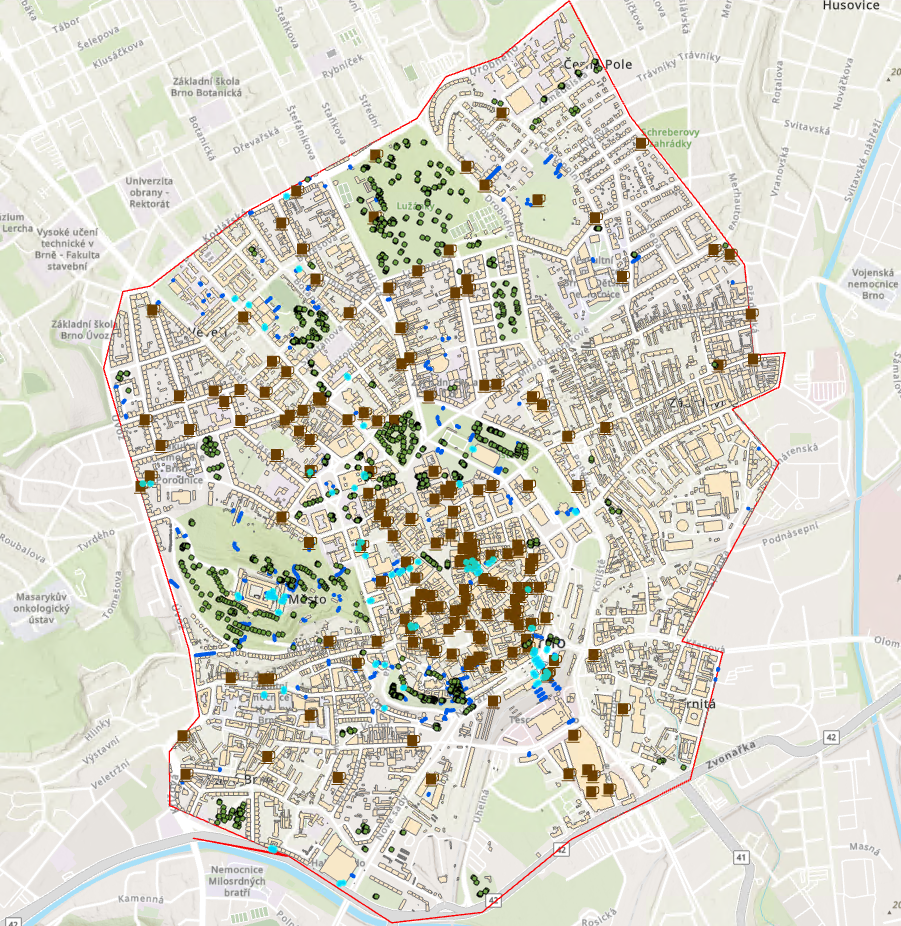
\includegraphics[width=\linewidth,height=0.8\textheight,keepaspectratio]{fig/current-pilot-study-area.png}
  \caption{Current pilot study area size}
  \label{fig:current-pilot-study-area}
\end{figure}

\end{document}
